\textcolor{red}{\section{Simulation}}
\label{sec:diss}

In the previous section we described the details of our multiple module approach for learning manipulation strategies. In this section, we evaluate this approach by a nonlinear and non-stationary control task in simulation.

\begin{figure}
  \centering
  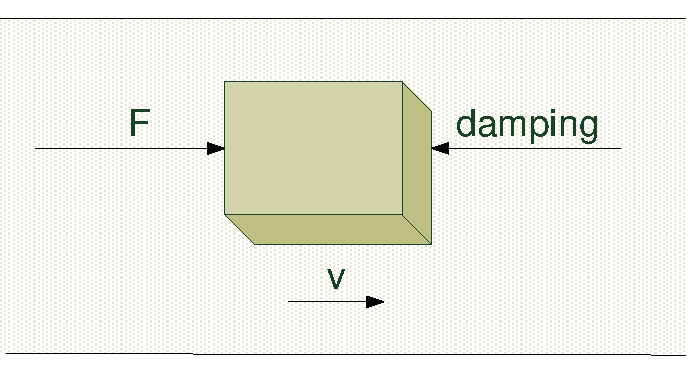
\includegraphics[width=7cm]{./fig/simulation.pdf}
  \caption{ \scriptsize{Illustration of the task. A object moves in an environment with changing damping. This can be understood as moving in a think liquid.}
}
\label{fig:simulation}
\end{figure}

We simulate an object moving in an environment with changing damping, e.g. a thick liquid (Figure~\ref{fig:simulation}). The target is to apply force onto the object so that it moves with constant speed. We simulate three different task contexts, i.e. three different damping conditions:

\begin{enumerate}
\item context 1: damping = $D$$v$
\item context 2: damping = $D$sin($v$)
\item context 3: damping = $D$tanh($v$)
\end{enumerate}
where $v$ is the object velocity and $D$ is the parameter of damping.

During the task execution, the task context randomly switches from one to another. This requires the controller to quickly realise and adapt to the changes. There is not an easy way to build a single module controller for such an environment without providing an explicit measure of damping as input. We apply our multiple module approach in this task to evaluate its efficiency. The simulator is performed in Matlab.
The mass of the object is set to be 5$N$, $D$ to be 15 $N.s/m$ and the target velocity is set to be 4$m/s$.

%The objective of this task is to learn an adaptive controller to move the object in a constant speed in the changing viscosity environment. During the task execution, the viscosity condition changes regularly from one to another and hence the learned controller has to quickly realise and adapt to the changes. As the viscosity is highly non-linear and the switches make the task non-stationary, this task is hard to be encoded by a single model. We use our multiple module approach to implement this task.

To learn a control policy of this system, we first demonstrate in the different task context. For each context, we generate three demonstrations by applying a sinusoidal varying force ($F$) to the object for a period of time. Randomly generated small noise is added to the force at each time step to simulate natural variability across the demonstrations. During the demonstrations, once the object starts to move, the force, previous velocity and current velocity $\{F_t, v_t, v_{t+1}\}$ are recoded. After recording the total 9 sets of demonstrations, we use DTW to compute the similarities between these demonstrations. The distance matrix is shown in Figure~\ref{fig:heatmap_sim}. As can be seen from the figure, the three task contexts can be clearly distinguished. This shows that by using this approach, different task context and their corresponding strategies can be properly separated into different modules.

\begin{figure}
  \centering
  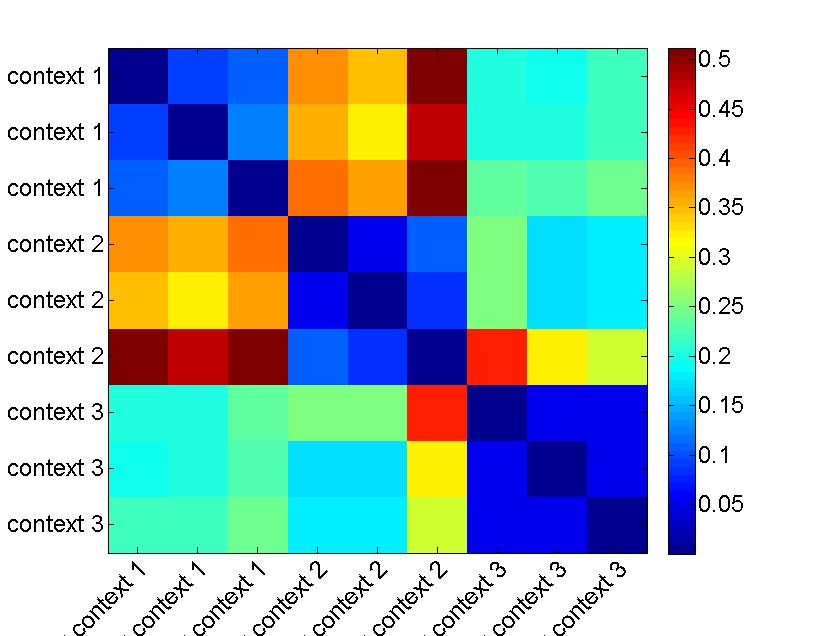
\includegraphics[width=7cm]{./fig/contexts.jpg}
  \caption{ \scriptsize{A heatmap representation of the distance matrix of 9 set of training data}
}
\label{fig:heatmap_sim}
\end{figure}

We hence group the demonstrations into 3 clusters and learn three modules for the task. As mentioned in the previous section, each modules is composed of a forward and an inverse model. In this task, the relation between the action and the state is always unique, hence we encode the forward and inverse models by the same GMM $\{F_t, v_t, v_{t+1}\mid \Omega\}$. With the forward model, we computed the expectation value of the next velocity $E\{v_{t+1}\mid \Omega,F_t,v_t\}$ by using GMR. The responsibility factors of each forward model are then computed according to the Equation~\ref{equ:lambda}. Finally, the motor commands are computed by the linear combination of the inverse models according to the Equation~\ref{e_mix}.

We apply the above mechanism to move the object. The damping of the environment is constantly switching across conditions.
Figure~\ref{fig:result_sim} shows the results. As can be seen from the figure, when the task context switches, the forward models can quickly recognize the correct context and hence guide the inverse models to produce the proper command to maintain the object velocity. After the switches, the object velocity can quickly be corrected to the target value. This simulation experiment shows that the proposed approach can indeed properly recognize the current task context and generate fast adaptive motor commands.

\begin{figure}
  \centering
  \subfloat[\scriptsize{Object velocity. The target velocity is 4m/s}]
  {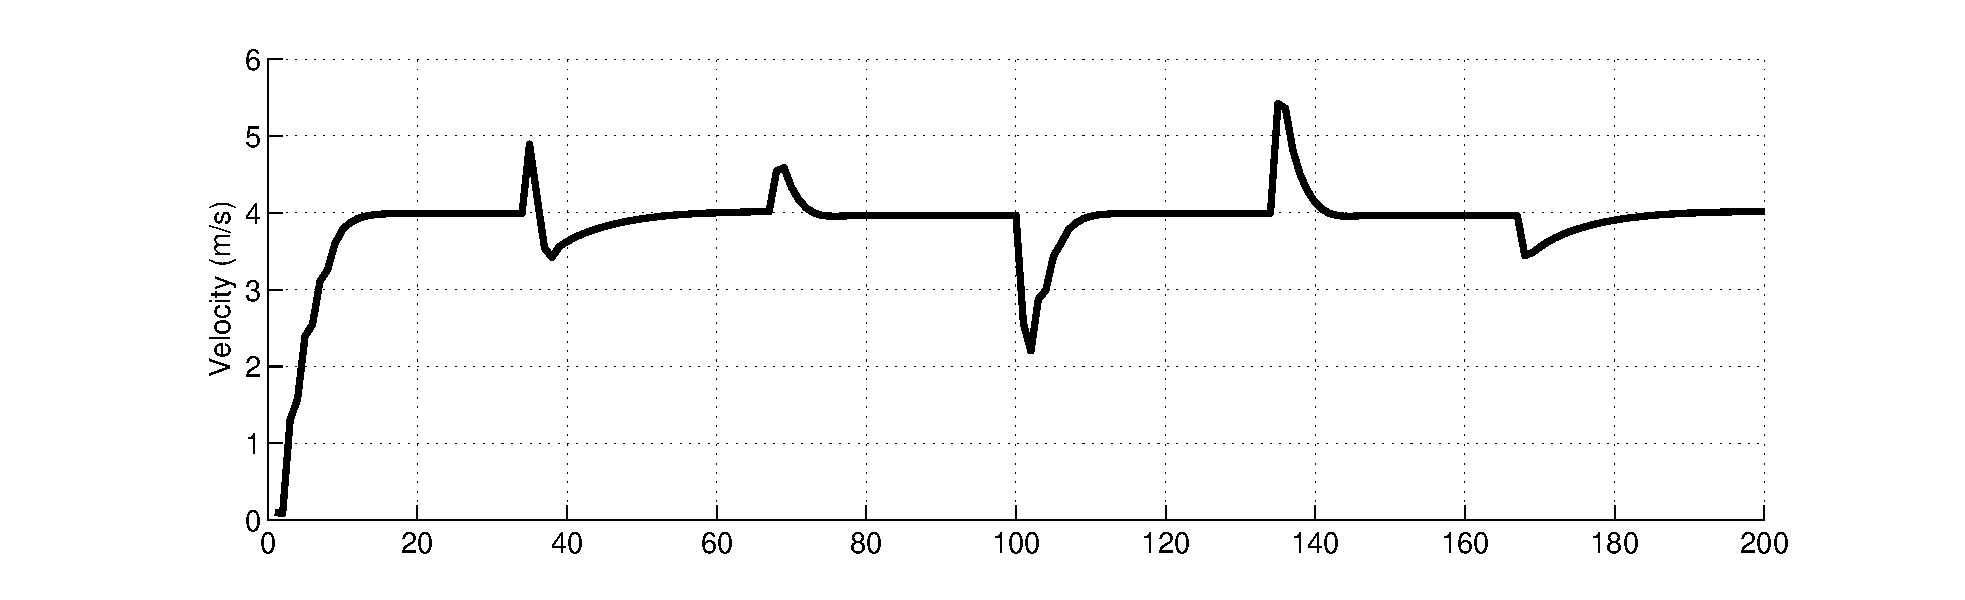
\includegraphics[width=8cm]{./fig/sim_vel.eps}}

  \vspace{0.3cm}
  %\vspace{0.5cm}
  \subfloat[\scriptsize{Force applied to object}]
  {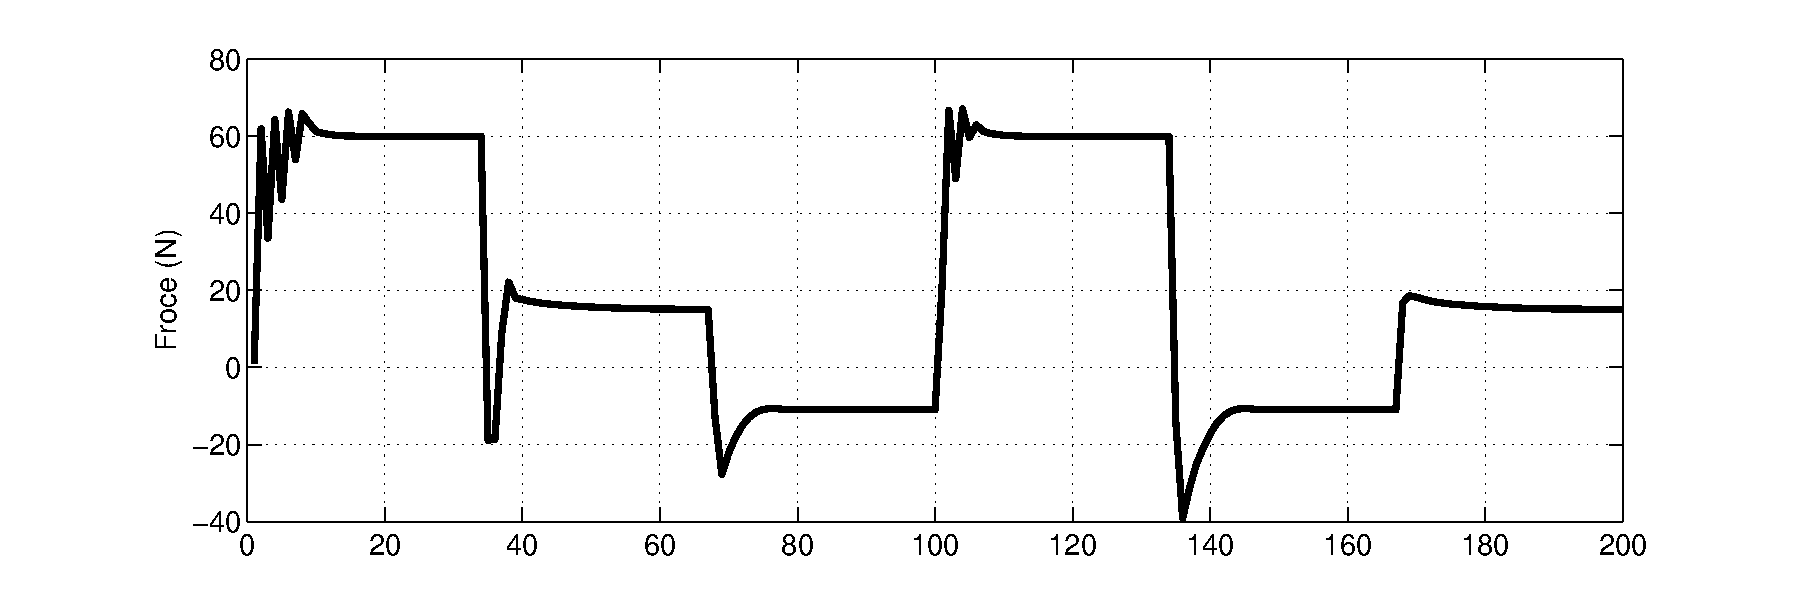
\includegraphics[width=8cm]{./fig/sim_force.eps}}

  \vspace{0.3cm}
  %\hspace{-0.5cm}
  \subfloat[\scriptsize{Responsibility factor for each module during task execution. The background colors represent the actual task context: pink-context 1, light blue-context 2 and light green-context 3.}]
  {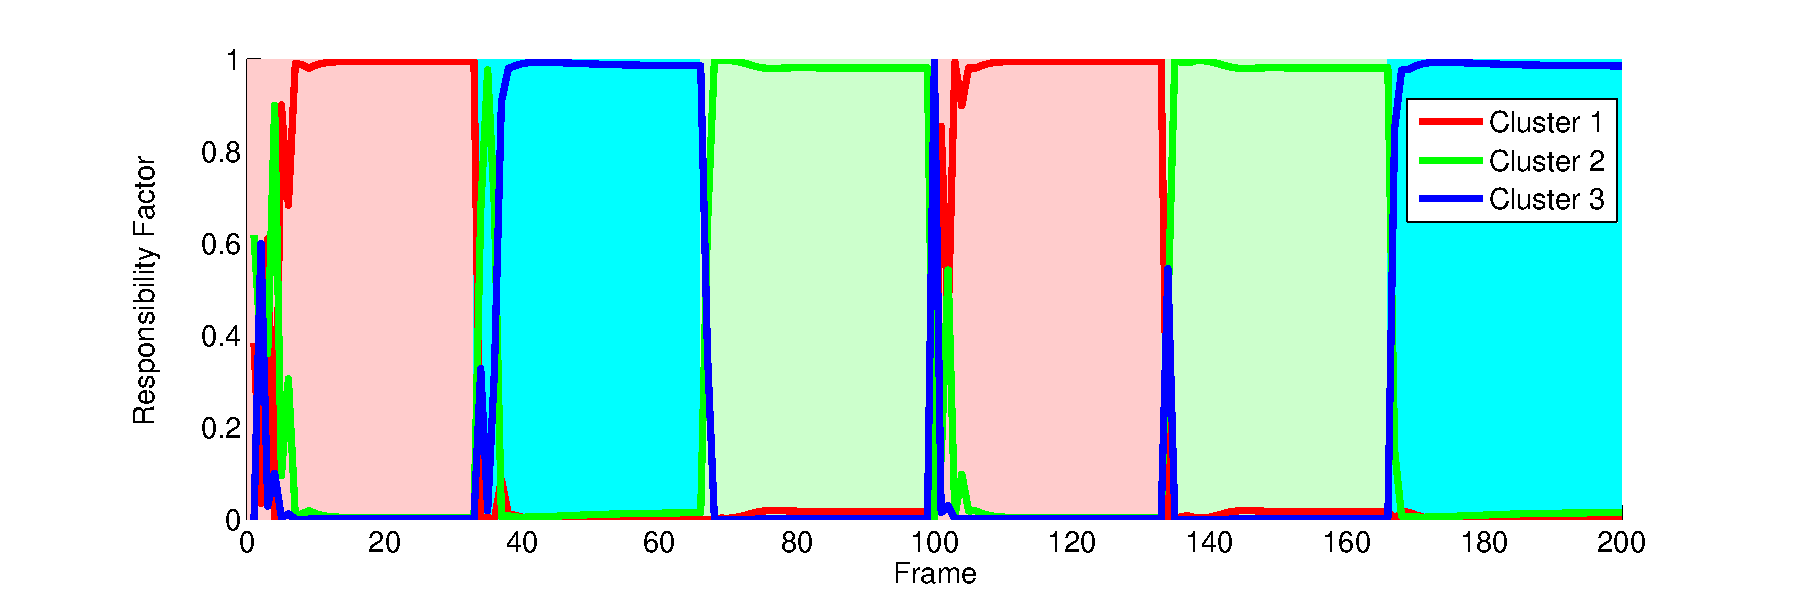
\includegraphics[width=8cm]{./fig/sim_rf2.eps}}
%
%  \vspace{0.3cm}
%  %\vspace{0.5cm}
%  \subfloat[\scriptsize{Actual task context}]
%  {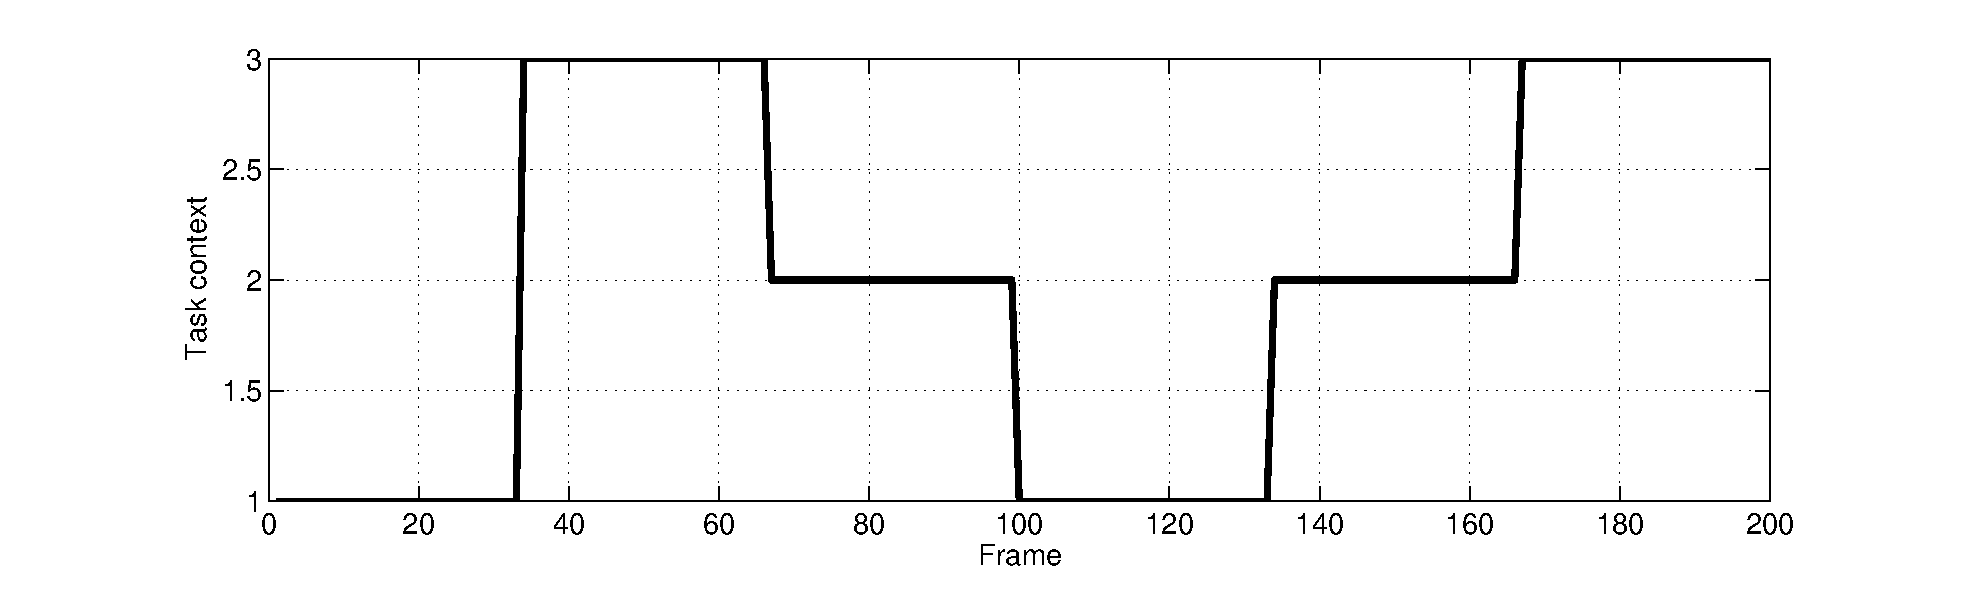
\includegraphics[width=8cm]{./fig/sim_context.eps}}

  \caption{ \scriptsize{Simulation results of moving an object in a changing environment}
}
\label{fig:result_sim}
\end{figure} 